\section{Auswertung}
\label{sec:Auswertung}

\subsection{Invertierter Verstärker}
\label{sec:Invertierter_Verstärker}
Die Verstärkung des invertierenden Linearverstärkers ist definiert als der Quotient aus dem Widerstand vor dem Eingang und jenem aus der Feedback-Schlleife, wie in \autoref{eq:Verstärkung} beschrieben.\\
Dadurch ergeben sich für die drei verwendeten Kombinationen aus Widerständen die Verstärkungen $V_{220} = 220$, $V_{150} = 150$ und $V_{100} = 100$.\\
Zur Bestimmung der Cutoff-Frequenzen der drei Aufbauten müssen die Daten zur unverstärkten und zur verstärkten Amplitude zur Bestimmung der Verstärkung mittels \autoref{eq:Verstärkung} herangezogen werden. Diese werden in einem doppelt logarithmischen Plot gegen die Frequenz aufgetragen.\\
Wie in \autoref{tab:ergebnisse_verstärkung_inverted} zu sehen ist, bleibt logarithmische Verstärkung bis zu einer gewissen Frequenz weitgehend konstant, bis sie einen gewissen Grenzfrequenzwert $f_\text{Grenz}$ erreicht. Ab diesem Wert fällt sie gegen die logarithmische Frequenz konstant ab.\\
Um die Cutoff-Frequenz zu bestimmen, müssen daher beiden Unterbereiche linear gefittet werden. Durch die Forderung, dass die beiden Ausgleichsgeraden sich bei der Cutoff-Frequenz treffen, ergibt sich für diese der Wert
\begin{aquation}
    \ln{\text{Grenz}} &= \frac{b-b^\prime}{a^\prime-a}
\end{aquation}
mit den Fitparametern $a^{(\prime)}$ und $b^{(\prime)}$ aus der Geradengleichung
\begin{aquation}
    \label{eq:linear_fit}
    \ln{V} &= a^{(\prime)}ln{f} + b^{(\prime)} \tp
\end{aquation}
Für den Fehler der Frequenz ergibt sich nach den Regeln der Differentialrechnung für die Cutoff-Frequenz der fortgepflanzte Fehler
\begin{aquation}
    \Delta f_\text{Grenz} &= \sqrt{\sum_{x = a^{(\prime)}, b^{(\prime)}} \left(\frac{\partial f_\text{Grenz}}{\partial x}\Delta x\right)^2} \tp
\end{aquation}
Die Leerlaufverstärkung $V_L$ ergibt sich als der Mittelwert der Messwerte bis zur Cutoff-Frequenz.\\
In \autoref{tab:ergebnisse_verstärkung_inverted} finden sich die Ergebnisse der so bestimmten Werte.

\begin{figure}
    \centering
    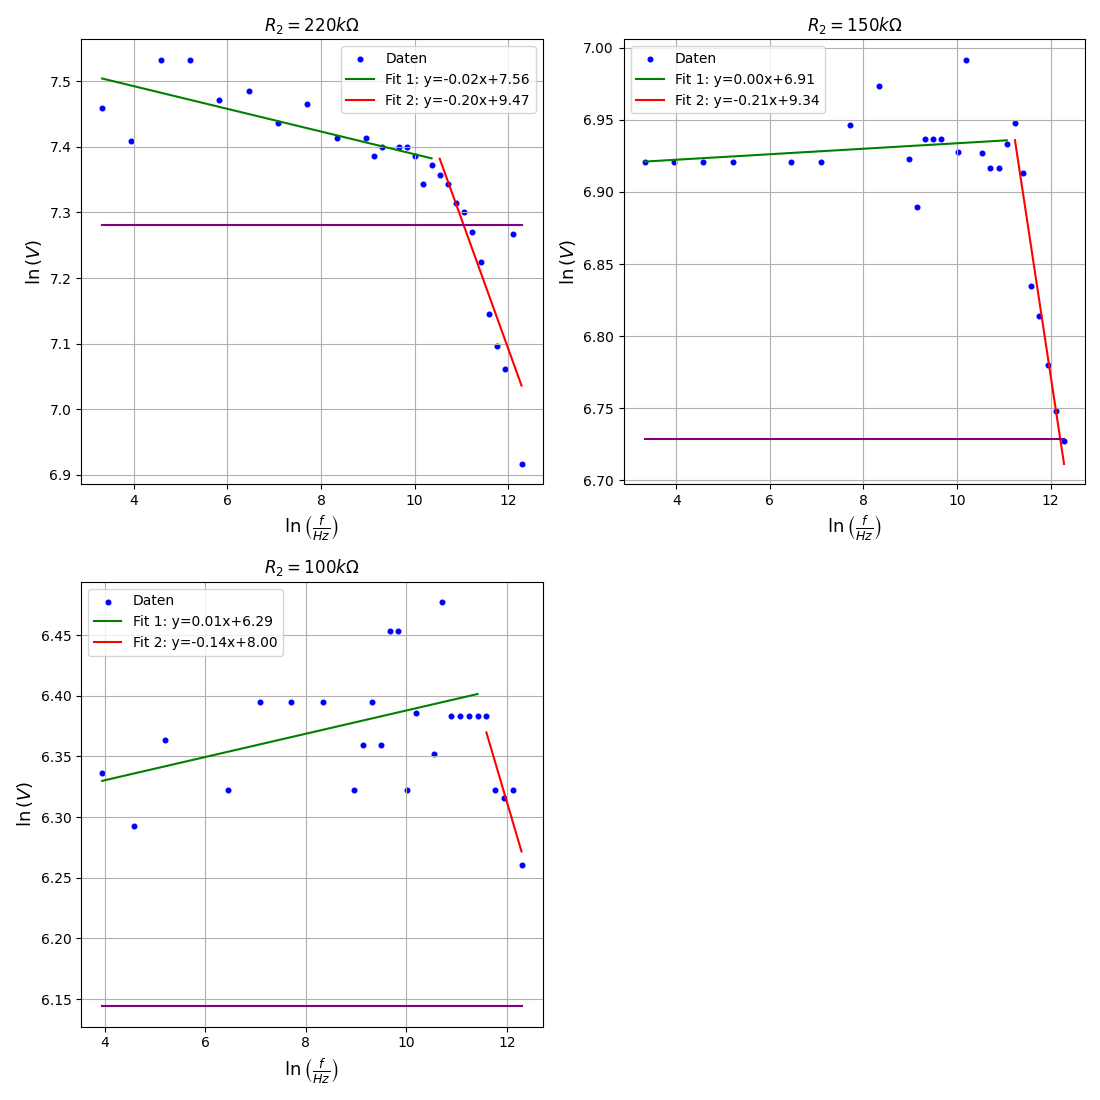
\includegraphics[width=\linewidth]{figures/inverted_gain.png}
        \caption{Doppelt logarithmische Plots der Verstärkung gegen die Frequenz beim invertierenden Verstärker. Der Widerstand $R_1$ in \autoref{fig:inverting-OpAmp} ist in allen Fällen $R_1 = 1\text{k$\Omega$}$.}
    \label{tab:ergebnisse_verstärkung_inverted}
\end{figure}

Die Phasen für den invertierten Verstärker sind in \autoref{tab:ergebnisse_phase_inverted} zu sehen.

\begin{figure}
    \centering
    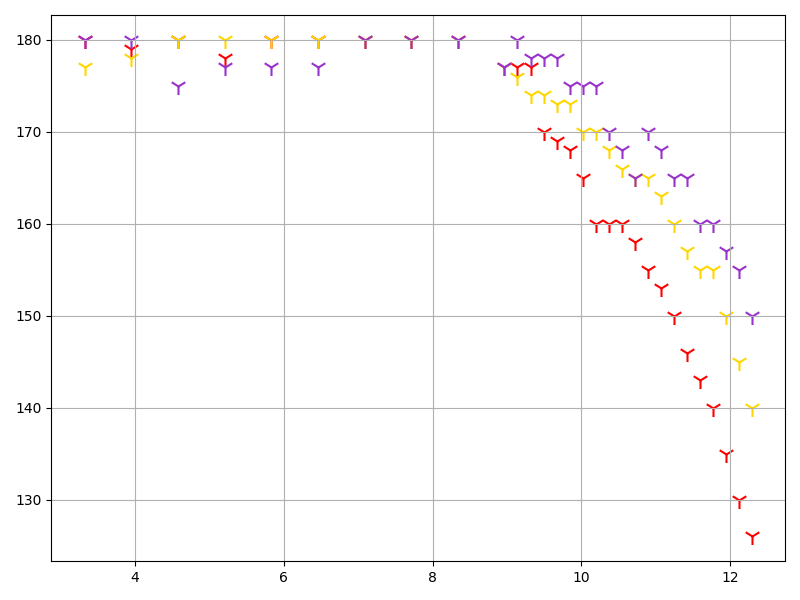
\includegraphics[width=0.6\linewidth]{figures/inverted_phase.png}
        \caption{Logarithmischer Plot der Phasen für die verschiedenen Widerstände gegen die Frequenz beim invertierenden Verstärker. Der Widerstand $R_1$ in \autoref{fig:inverting-OpAmp} ist in allen Fällen $R_1 = 1\text{k$\Omega$}$.}
    \label{tab:ergebnisse_phase_inverted}
\end{figure}

\begin{table}[h!]
    \centering
    \begin{tabular}{|>{$}c<{$}|>{$}c<{$}|>{$}c<{$}|>{$}c<{$}|}
    \hline
    V_{\text{Theorie}} & V_{\text{Leerlauf}} & f_\text{Grenz} \text{ / kHz} & f_\text{Grenz} \cdot V \text{ / MHz}\\ \hline
    220 & 174.64 \pm 2.61 & 31.7 \pm 0.7 & 5.53 \pm 0.20 \\
    150 & 123.26 \pm 1.29 & 64.7 \pm 3.0 & 7.97 \pm 0.45 \\
    100 & 84.70 \pm 1.04 & 82.6 \pm 14.0 & 7.00 \pm 1.37 \\
    \hline
    \end{tabular}
    \caption{Titel der Tabelle}
    \label{tab:ergebnisse_verstärkung_inverted}
\end{table}

\subsection{Integrator und Differentiator}
Für den Integrator ergibt sich mit $R = 10\text{k$\Omega$}$ und $C = 100 \text{nF}$ die theoretische Zeitkonstante 
\begin{aquation}
    {RC}_\text{$\int$,theo} &= 1 \text{ms} \tp
\end{aquation}
Für den Differentiator ergibt sich als Theoriewert mit $R = 10\text{k$\Omega$}$ $C = 22 \text{nF}$
\begin{aquation}
    {RC}_\text{$\partial$,theo} &= 22 \text{ms} \tp
\end{aquation}
Durch Fitten der Daten in einem doppelt logarithmischen Plot nach \autoref{eq:linear_fit}, wie in \autoref{fig:integrator_differentiator} gezeigt, ergibt sich für die Berechnung der Zeitkonstante des Integrators 
\begin{aquation}
    RC &= e^{-b} &= (8.90 \pm 0.27) \text{ms}
\end{aquation}
und für die Zeitkonstante des Differentiators analog 
\begin{aquation}
    RC &= e^{b} &= (79.85 \pm 10.98) \text{ms} \tp 
\end{aquation}
Die Fitparameter sind 
\begin{aquation}
    a_{\int} &= -0.84 \pm 0.03 \\
    b_{\int} &= 4.72 \pm 0.03
\end{aquation}
und 
\begin{aquation}
    a_\partial &= 1.04 \pm 0.10 \\
    b_\partial &= 2.53 \pm 0.14 \tp
\end{aquation}
\begin{figure}
    \centering
    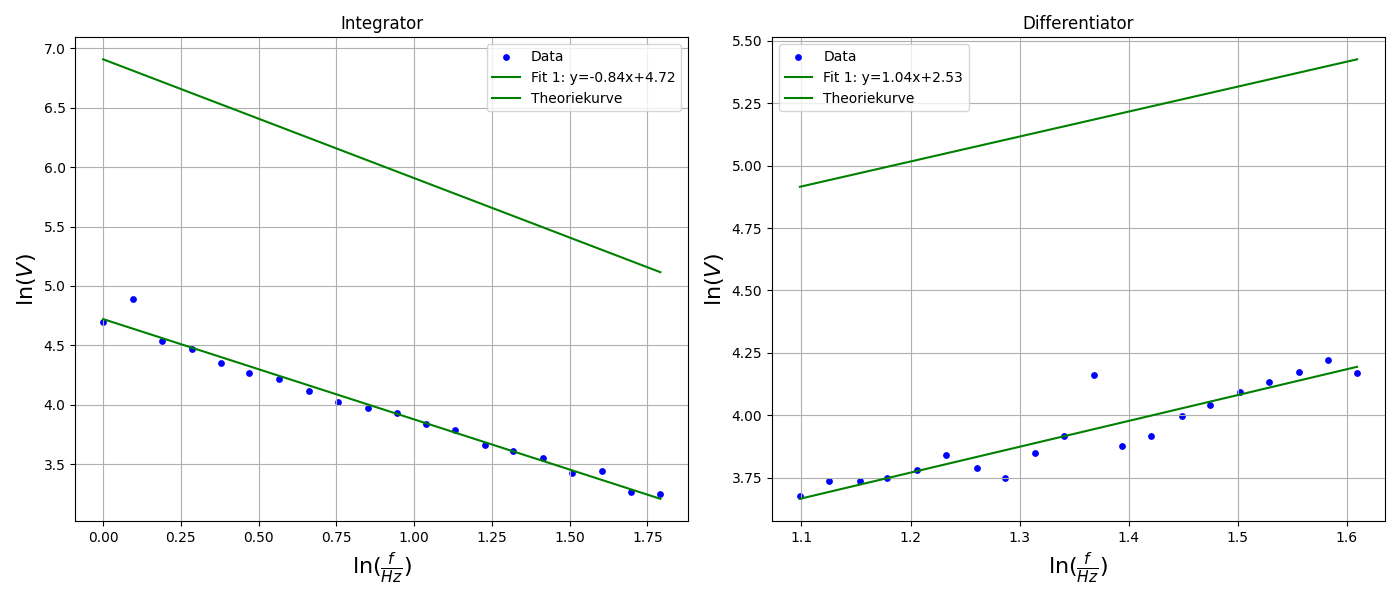
\includegraphics[width=\linewidth]{figures/Int+Diff.png}
        \caption{Doppelt logarithmische Plots der Verstärkung gegen die Frequenz bei Integrator und Differentiator.}
    \label{fig:integrator_differentiator}
\end{figure}